\chapter{Microbiomes and Symbioses}\label{ch:b3:microbiomes}

You carry about thirty-eight trillion bacteria, roughly one for every
cell of your own, most of them in the last metre of your gut, where
they weigh about as much as your brain and carry a hundred times more
genes than you do. A mouse raised without any of them needs a third
more food to keep its weight, has a stunted immune system, and behaves
oddly. A pea plant feeds a tenth of its sugar to bacteria in nodules on
its roots and gets its nitrogen in return; four fifths of all land
plants trade sugar for phosphate with fungi wrapped around their roots,
as they have for four hundred million years; a coral is an animal that
farms algae inside its cells and dies when the sea warms enough to make
it evict them. Living things are not individuals but consortia, and
this chapter treats the biology of the partnerships: how they are
counted and characterised by sequencing, what the partners exchange,
how the exchange is negotiated and policed, and why some partners end
up as organelles.

\section{Words for living together}

\begin{definition}[Symbiosis]\label{def:b3:microbiomes:symbiosis}
\index{symbiosis}\index{mutualism}\index{commensalism}\index{holobiont}\index{microbiome}\index{vertical transmission}
\emph{Symbiosis} is the sustained, intimate association of organisms of
different species; it is a \emph{mutualism} if both gain, a
\emph{commensalism} if one gains and the other is unaffected, and a
parasitism if one gains at the other's expense --- and the same pair
may move along that line with circumstances. An \emph{endosymbiont}
lives inside its host's cells; an \emph{obligate} partner cannot live
alone. Symbionts are transmitted \emph{vertically}, from parent to
offspring (the aphid's \emph{Buchnera} pass through the egg), or
\emph{horizontally}, acquired anew each generation from the environment
or from other hosts (the squid's \emph{Vibrio}, the human gut's
bacteria). The \emph{microbiome} is the whole community of microbes of
a habitat --- a gut, a leaf surface, a gram of soil --- and the
\emph{holobiont} is a host together with its microbiome, considered as
the unit that natural selection sees.
\end{definition}

\begin{example}[Three obligate partners]\label{ex:b3:microbiomes:obligate}
The aphid \emph{Buchnera} has lived inside its host's cells for two
hundred million years, makes the essential amino acids that phloem sap
lacks, and has shrunk its genome to \qty{640}{kb} --- a seventh of its
free-living relatives' --- losing every gene the host now supplies. The
bacterium \emph{Wolbachia}, in two thirds of insect species, is
transmitted through eggs only, and so has evolved to favour females: it
kills male embryos, feminises them, or makes uninfected females' eggs
die when fertilised by infected males (\emph{cytoplasmic
incompatibility}), which spreads it through a population; mosquitoes
carrying it transmit dengue poorly, and releasing them has cut dengue
in several cities. The amoeba \emph{Paulinella} took in a
cyanobacterium about a hundred million years ago that is now neither
quite a bacterium nor quite a chloroplast --- a second, independent
origin of photosynthetic organelles, caught halfway.
\end{example}

\section{Counting a community}

\begin{method}[Profiling a microbiome by sequencing]\label{met:b3:microbiomes:16s}
\index{16S rRNA sequencing}\index{metagenomics}\index{operational taxonomic unit}
Most microbes cannot be cultured; they are counted by their DNA. (1)
Extract DNA from the sample --- faeces, soil, seawater filtered onto a
membrane. (2) Either amplify the gene for the small-subunit ribosomal
RNA (\emph{16S}) with \omterm{def:b3:genetic-engineering:pcr}{primers} matching its universal regions, and
sequence the variable regions between them --- an \emph{amplicon}
survey, cheap, which identifies bacteria to about the genus and counts
them by read number; or sequence all the DNA --- \emph{shotgun
metagenomics}, which recovers genes and whole genomes and so reports
what the community can do, not only who is there. (3) Cluster the reads
into sequence variants or \emph{\omterm{met:b3:microbiomes:16s}{operational taxonomic units}} (OTUs,
conventionally at \qty{97}{\%} identity for a ``species''), assign them
by comparison with databases (\cref{ch:b3:bioinformatics}), and
tabulate counts per sample. (4) Compute diversity within a sample and
compare composition between samples. The counts are relative --- a
sample's reads sum to a fixed total --- and are biased by extraction,
\omterm{def:b3:genetic-engineering:pcr}{primers} and copy number, so differences between samples processed the
same way are trustworthy where absolute numbers are not.
\end{method}

\begin{definition}[Diversity]\label{def:b3:microbiomes:diversity}
\index{species richness}\index{Shannon index}\index{Simpson index}\index{rarefaction}
For a community of $S$ species with relative abundances $p_{1},\dots,
p_{S}$ ($\sum p_{i} = 1$): the \emph{richness} is $S$; the
\emph{Shannon index} $H = -\sum_{i} p_{i}\ln p_{i}$ measures the
uncertainty about the species of a randomly drawn individual, and
$e^{H}$ is the number of equally abundant species that would give the
same uncertainty (the effective number of species); the \emph{Simpson
index} $D = \sum_{i} p_{i}^{2}$ is the probability that two individuals
drawn at random are of the same species, and $1/D$ is another
effective number, weighted toward the common species. Richness depends
on how many individuals one has looked at: a \emph{rarefaction curve}
plots the species found against the number of individuals sampled, and
flattens when most species have been seen.
\end{definition}

\begin{theorem}[Rarefaction]\label{thm:b3:microbiomes:rarefaction}
\index{rarefaction!formula}\index{Good's coverage}
A sample contains $N$ individuals of $S$ species, $N_{i}$ of species
$i$. The expected number of species in a random subsample of $n$
individuals, drawn without replacement, is
\[
E[S_{n}] = \sum_{i=1}^{S}\left[1 - \frac{\binom{N - N_{i}}{n}}
{\binom{N}{n}}\right],
\]
which rises with $n$ and equals $S$ at $n = N$. Two samples of
different sizes are compared by rarefying both to the same $n$. The
fraction of the community's individuals belonging to species not yet
seen is estimated by \emph{\omterm{thm:b3:microbiomes:rarefaction}{Good's coverage}}: about $f_{1}/N$, where
$f_{1}$ is the number of species seen exactly once (singletons).
\end{theorem}
\begin{proof}
Species $i$ is absent from the subsample exactly when all $n$
individuals are drawn from the $N - N_{i}$ others, which happens in
$\binom{N - N_{i}}{n}$ of the $\binom{N}{n}$ equally likely subsamples;
so species $i$ is present with probability $1 - \binom{N-N_{i}}{n}/
\binom{N}{n}$, and the expected count of species present is the sum of
these probabilities (expectation of a sum of indicators). Each term
increases with $n$, and at $n = N$ every binomial in the numerator is
zero. Good's estimate: an individual drawn next belongs to an unseen
species with about the probability that a randomly chosen individual
of the sample was the only one of its kind, $f_{1}/N$ (Good, 1953);
its justification is admitted here.
\end{proof}

\begin{example}[Two guts]\label{ex:b3:microbiomes:two-guts}
A sample of $1000$ reads from one person yields $150$ species, with
$H = 3.5$ and $40$ singletons; a sample of $5000$ reads from another
yields $260$ species. The second is not necessarily more diverse: it
was sampled five times more deeply, and rarefying it to $1000$ reads
may give $150$ too. The first sample's coverage is $1 - 40/1000 =
\qty{96}{\%}$: four per cent of the bacteria in that gut belong to
species the sample never saw, and a deeper sample will find them.
Effective numbers, $e^{3.5} \approx 33$ species' worth of evenness
against a richness of $150$, say that a few species dominate --- which
is how every gut looks.
\end{example}

\begin{omfigure}
\begin{tikzpicture}
\begin{axis}[
  width=0.68\linewidth, height=5.6cm,
  axis x line=bottom, axis y line=left,
  xmin=0, xmax=5000, ymin=0, ymax=300,
  xlabel={reads sampled, $n$}, ylabel={species observed},
  xlabel style={font=\small, at={(axis description cs:0.5,-0.12)}, anchor=north}, ylabel style={font=\small},
  tick label style={font=\small}, xtick={0,1000,2000,3000,4000,5000}, ytick={0,100,150,200,260},
  clip=false,
]
\addplot[very thick, omDef, domain=0:5000, samples=60] {260*(1-exp(-x/1500))};
\addplot[very thick, omThm, domain=0:1000, samples=30] {150*(1-exp(-x/300))*1.0};
\addplot[very thick, omThm, dashed, domain=1000:5000, samples=30] {150*(1-exp(-x/300))*1.0 + 8*(1-exp(-(x-1000)/2000))};
\draw[dashed, gray] (axis cs:1000,0) -- (axis cs:1000,300);
\node[font=\scriptsize, omDef, anchor=north west] at (axis cs:1200,292) {second gut: $260$ species at $5000$ reads};
\node[font=\scriptsize, omThm, anchor=north east] at (axis cs:4900,140) {first gut: $150$ at $1000$, near its plateau};
\node[font=\scriptsize, gray, anchor=south west] at (axis cs:1050,10) {rarefy here to compare};
\end{axis}
\end{tikzpicture}

{\small \omterm{def:b3:microbiomes:diversity}{Rarefaction} curves. Species found rise with the reads sampled
and flatten as the community is exhausted; two samples are compared at
the same depth. Here the second gut is still climbing at $5000$ reads,
so its true richness is higher still.}
\end{omfigure}

\section{The human microbiome}

\begin{definition}[The gut community]\label{def:b3:microbiomes:gut}
\index{gut microbiome}\index{short-chain fatty acid}\index{colonisation resistance}\index{dysbiosis}
The human gut holds about $4\times 10^{13}$ bacteria, nearly all in the
colon at $10^{11}$ per gram of contents, against $10^{3}$ per gram in
the acid stomach and $10^{4}$--$10^{7}$ along the small intestine, whose
flow is fast and whose bile is hostile. Some five hundred to a thousand
species per person, most from two phyla, the Bacteroidetes and the
Firmicutes, nearly all anaerobes; each person's set is distinct and
stable for years, fixed largely in the first three years of life from
the mother and the household. What they do: ferment the fibre that
human enzymes cannot digest into \emph{short-chain fatty acids} ---
acetate, propionate, butyrate --- which feed the colon's own cells and
supply up to a tenth of the host's calories; make vitamin~K and some B
vitamins; transform bile acids and drugs; occupy every niche so that an
invader finds no foothold (\emph{colonisation resistance}); and train
the immune system, whose regulatory T~cells and IgA-secreting cells
develop in response to them (\cref{ch:b3:adaptive-immunity}). A
community shifted away from this state --- fewer species, fewer
fermenters, more facultative aerobes --- is a \emph{dysbiosis}, seen in
inflammatory bowel disease, after \omterm{def:b3:bacteriology:antibiotics}{antibiotics}, and in obesity, though
which is cause and which effect is usually unclear.
\end{definition}

\begin{proof}[Evidence]
Mice raised germ-free in sterile isolators (Gordon and colleagues,
2000s) have thin intestinal walls, small lymphoid organs, low levels of
antibody, and need \qty{30}{\%} more calories to maintain their weight;
colonised with a normal mouse microbiota they gain fat within two
weeks. Given the microbiota of an obese mouse rather than a lean one,
germ-free mice gained more fat on the same food (Turnbaugh, 2006): the
community itself affects energy harvest. In humans, recurrent
\emph{Clostridioides difficile} colitis --- a \omterm{def:b3:microbiomes:gut}{dysbiosis} in which
\omterm{def:b3:bacteriology:antibiotics}{antibiotics} have cleared the competitors of a toxin-producing spore
former --- was cured in \qty{94}{\%} of patients by infusion of a
healthy donor's faeces, against \qty{31}{\%} with the standard
\omterm{def:b3:bacteriology:antibiotics}{antibiotic} (van~Nood, 2013), the first randomised trial in which a
community, not a molecule, was the drug.
\end{proof}

\begin{omfigure}
\begin{tikzpicture}
\begin{axis}[
  width=0.68\linewidth, height=5.4cm,
  ybar, bar width=18pt,
  axis x line=bottom, axis y line=left,
  ymode=log, ymin=1, ymax=1e13,
  symbolic x coords={stomach, duodenum, jejunum, ileum, colon},
  xtick=data, ytick={1e1,1e3,1e5,1e7,1e9,1e11},
  ylabel={bacteria per gram of contents},
  ylabel style={font=\small}, tick label style={font=\small},
  clip=false,
]
\addplot[fill=omDef!40, draw=omDef] coordinates {(stomach,1e3) (duodenum,1e4) (jejunum,1e5) (ileum,1e7) (colon,1e11)};
\node[font=\scriptsize, anchor=west, xshift=10pt] at (axis cs:stomach,3e3) {acid, pH 2};
\node[font=\scriptsize, anchor=south] at (axis cs:jejunum,1.5e5) {bile, fast flow};
\node[font=\scriptsize, anchor=south, align=center] at (axis cs:colon,1.5e11) {slow, anaerobic:\\the fermenter};
\end{axis}
\end{tikzpicture}

{\small Bacterial density along the human gut, on a logarithmic scale:
a hundred-million-fold rise from the acid stomach to the colon, where
nearly all of the body's microbes live.}
\end{omfigure}

\begin{omfigure}
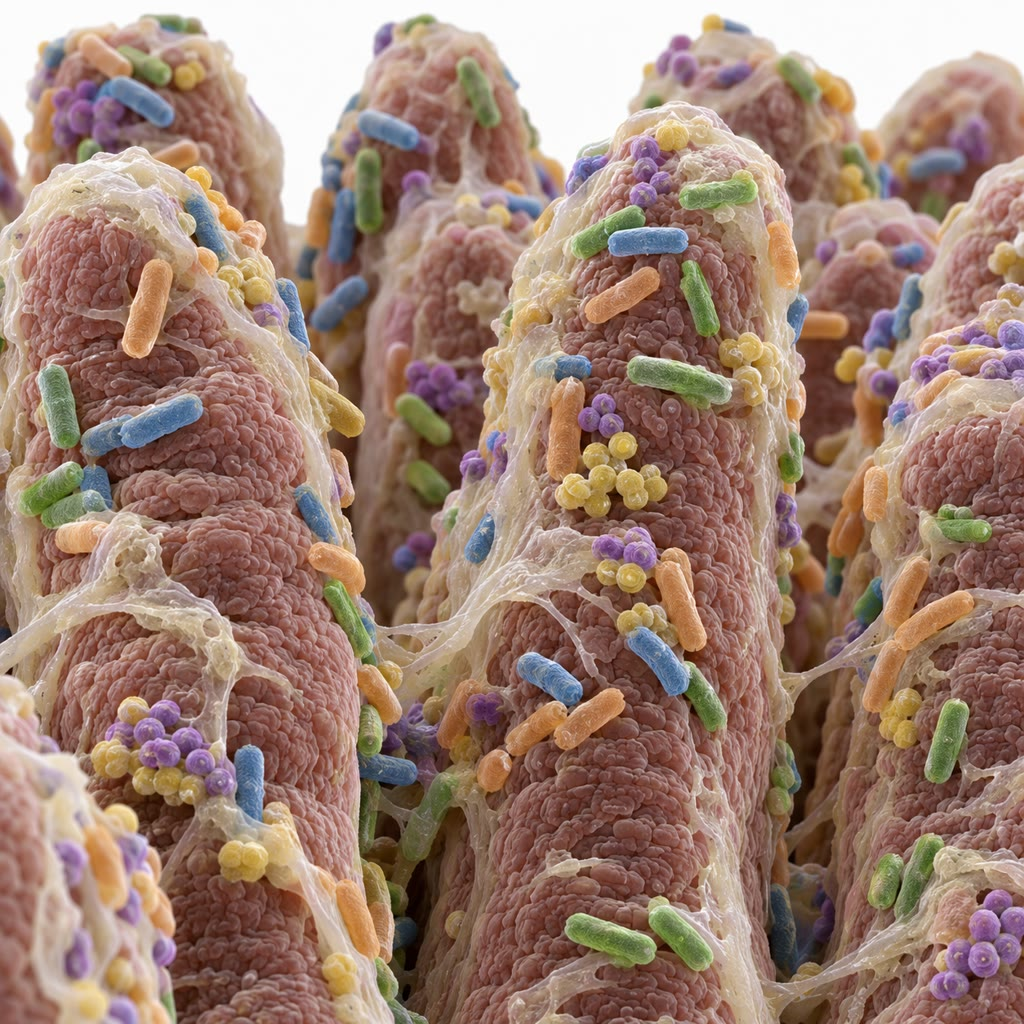
\includegraphics[width=0.40\linewidth]{images/book5/ai/b5-14-gut-microbiota.jpg}

{\small The surface of the intestinal lining in the scanning electron
microscope, bacteria of several kinds lodged in the mucus between the
villi.}
\end{omfigure}

\section{Plants and their partners}

\begin{definition}[The legume--rhizobium symbiosis]\label{def:b3:microbiomes:nodule}
\index{rhizobia}\index{root nodule}\index{Nod factor}\index{leghaemoglobin}\index{nitrogenase}
Legumes house nitrogen-fixing bacteria (\emph{rhizobia}) in \emph{root
nodules}, organs built for the purpose after a molecular dialogue. The
root secretes flavonoids; a rhizobium of the matching species answers
with \emph{Nod factors} --- lipochitooligosaccharides whose decorations
specify the partner; a receptor kinase on the root hair binds them and
triggers oscillations of calcium in the nucleus, the curling of the
root hair around the bacteria, and an \emph{infection thread} that
grows inward through the cells while the cortex below begins to divide
into a nodule. The bacteria are released into the nodule cells inside
membranes and differentiate into \emph{bacteroids} that express
\emph{nitrogenase}, the enzyme that reduces N$_{2}$ to ammonia at the
cost of sixteen ATP per molecule. Nitrogenase is destroyed by oxygen,
yet the bacteroids respire hard; the nodule solves the contradiction
with a diffusion barrier and with \emph{leghaemoglobin}, a plant
haemoglobin that binds oxygen tightly and ferries it to the bacteroids
at a low free concentration --- it is what makes a cut nodule pink. The
plant pays six to ten per cent of its photosynthate and receives most
of its nitrogen; the fixed nitrogen of the world's legume crops
approaches that of the fertiliser industry.
\end{definition}

\begin{omfigure}
\begin{tikzpicture}[every node/.style={font=\scriptsize}, >=stealth]
  % stage 1: root hair and bacteria, flavonoid / Nod factor exchange
  \begin{scope}
    \draw[thick, omMeth!60!black, fill=omMeth!15] (0,0) rectangle (1.2,3.0);
    \draw[thick, omMeth!60!black, fill=omMeth!15] (1.2,1.6) .. controls (2.4,1.7) and (2.6,2.6) .. (2.9,2.4) .. controls (2.5,2.3) and (2.3,1.4) .. (1.2,1.2) -- cycle;
    \foreach \p in {(3.1,2.7),(3.4,2.3),(3.3,1.9)} \fill[omProp] \p ellipse (0.14 and 0.07);
    \draw[->, omMeth!60!black, thick] (2.6,1.5) -- (3.2,1.4); \node[below, omMeth!60!black] at (3.0,1.35) {flavonoids};
    \draw[<-, omProp, thick] (2.5,2.85) -- (3.0,3.0); \node[above, omProp] at (2.4,2.95) {Nod factors};
    \node[below, align=center] at (1.6,-0.2) {1. dialogue: root hair\\and rhizobia};
  \end{scope}
  % stage 2: curled hair, infection thread
  \begin{scope}[xshift=4.6cm]
    \draw[thick, omMeth!60!black, fill=omMeth!15] (0,0) rectangle (1.2,3.0);
    \draw[thick, omMeth!60!black, fill=omMeth!15] (1.2,1.6) .. controls (2.3,1.8) and (2.8,2.6) .. (2.2,2.8) .. controls (1.9,2.9) and (1.8,2.5) .. (2.0,2.4) .. controls (2.3,2.2) and (1.9,1.3) .. (1.2,1.2) -- cycle;
    \draw[omProp, very thick] (2.05,2.55) .. controls (1.8,2.1) and (1.4,1.7) .. (0.4,1.3);
    \foreach \p in {(1.85,2.3),(1.5,1.9),(1.1,1.6),(0.7,1.4)} \fill[omProp] \p ellipse (0.1 and 0.05);
    \node[right, omProp, font=\tiny] at (2.3,1.0) {infection thread};
    \foreach \p in {(0.3,0.5),(0.6,0.7),(0.9,0.5)} \draw[omMeth!60!black] \p circle (0.12);
    \node[below, align=center] at (1.6,-0.2) {2. hair curls; thread grows in;\\cortex cells divide};
  \end{scope}
  % stage 3: nodule
  \begin{scope}[xshift=9.0cm]
    \draw[thick, omMeth!60!black, fill=omMeth!15] (0,0) rectangle (1.2,3.0);
    \draw[thick, omThm!60!black, fill=omThm!25] (1.2,1.5) ellipse (1.3 and 1.0);
    \foreach \p in {(1.0,1.5),(1.5,1.8),(1.6,1.2),(1.1,1.9),(1.2,1.1),(2.0,1.5)} \fill[omProp] \p circle (0.1);
    \node[right, align=left] at (2.6,2.0) {nodule: bacteroids\\with nitrogenase};
    \node[right, align=left, omThm!60!black] at (2.6,1.1) {pink: leghaemoglobin\\keeps O$_2$ low};
    \draw[->, thick] (0.6,2.4) -- (1.0,2.0) node[pos=0, above] {sugar};
    \draw[<-, thick] (0.6,0.6) -- (1.0,1.0) node[pos=0, below] {NH$_3$};
    \node[below, align=center] at (1.6,-0.2) {3. bacteroids fix N$_2$;\\sugar for ammonia};
  \end{scope}
\end{tikzpicture}

{\small Making a nodule. Flavonoids from the root and \omterm{def:b3:microbiomes:nodule}{Nod factors} from
the rhizobium identify the partners; the root hair curls, an infection
thread carries the bacteria inward, and the cortex builds a nodule in
which bacteroids, kept at low oxygen by \omterm{def:b3:microbiomes:nodule}{leghaemoglobin}, fix nitrogen
for sugar.}
\end{omfigure}

\begin{definition}[Mycorrhizas]\label{def:b3:microbiomes:mycorrhiza}
\index{mycorrhiza}\index{arbuscular mycorrhiza}\index{common symbiosis pathway}
\emph{Mycorrhizas} are associations of roots with fungi, found in some
\qty{80}{\%} of plant species and in the earliest land-plant fossils.
In \emph{arbuscular mycorrhizas} the fungus (a Glomeromycete) enters
the root cells and branches into a tree-like arbuscule across which
phosphate, nitrogen and water pass to the plant and sugars and lipids
to the fungus; the fungal hyphae extend the absorbing surface of the
root a hundredfold and reach phosphate the root cannot. In
\emph{ectomycorrhizas}, of forest trees, the fungus sheathes the root
and grows between the cells. The plant genes that admit the fungus are
the same \emph{common \omterm{def:b3:microbiomes:symbiosis}{symbiosis} pathway} --- receptor, calcium spiking,
transcription factors --- that legumes reuse for \omterm{def:b3:microbiomes:nodule}{rhizobia}: the nodule
is a late invention built on a fungal partnership four hundred million
years older.
\end{definition}

\begin{proposition}[Trade and its policing]\label{prop:b3:microbiomes:sanctions}
\index{partner choice}\index{sanctions}\index{cheater}
A \omterm{def:b3:microbiomes:symbiosis}{mutualism} is an exchange, and each partner is selected to give less
and take more; it persists because the other partner can retaliate.
Legumes restrict oxygen to nodules whose \omterm{def:b3:microbiomes:nodule}{rhizobia} fix no nitrogen,
halving their reproduction (Kiers, 2003): \emph{sanctions}. Plants in
mycorrhizal networks allocate more carbon to the fungal partners that
deliver more phosphate, and the fungi more phosphate to the roots that
pay more carbon --- a market in which both sides reward the better
trader (Kiers, 2011). Squid expel light-organ bacteria that do not
glow; humans' immune systems tolerate the commensals that stay in the
lumen and attack those that cross the wall. Where a host can neither
choose nor sanction --- an endosymbiont inherited through the egg ---
the alignment of interests comes instead from shared fate: a
vertically transmitted symbiont reproduces only when its host does,
and selection on the symbiont favours the host's reproduction. The
mode of transmission thus predicts the character of the partnership:
\omterm{def:b3:microbiomes:symbiosis}{vertical transmission} toward \omterm{def:b3:microbiomes:symbiosis}{mutualism} and dependence, horizontal
transmission toward exploitation held in check by policing.
\end{proposition}
\admitted

\begin{omfigure}
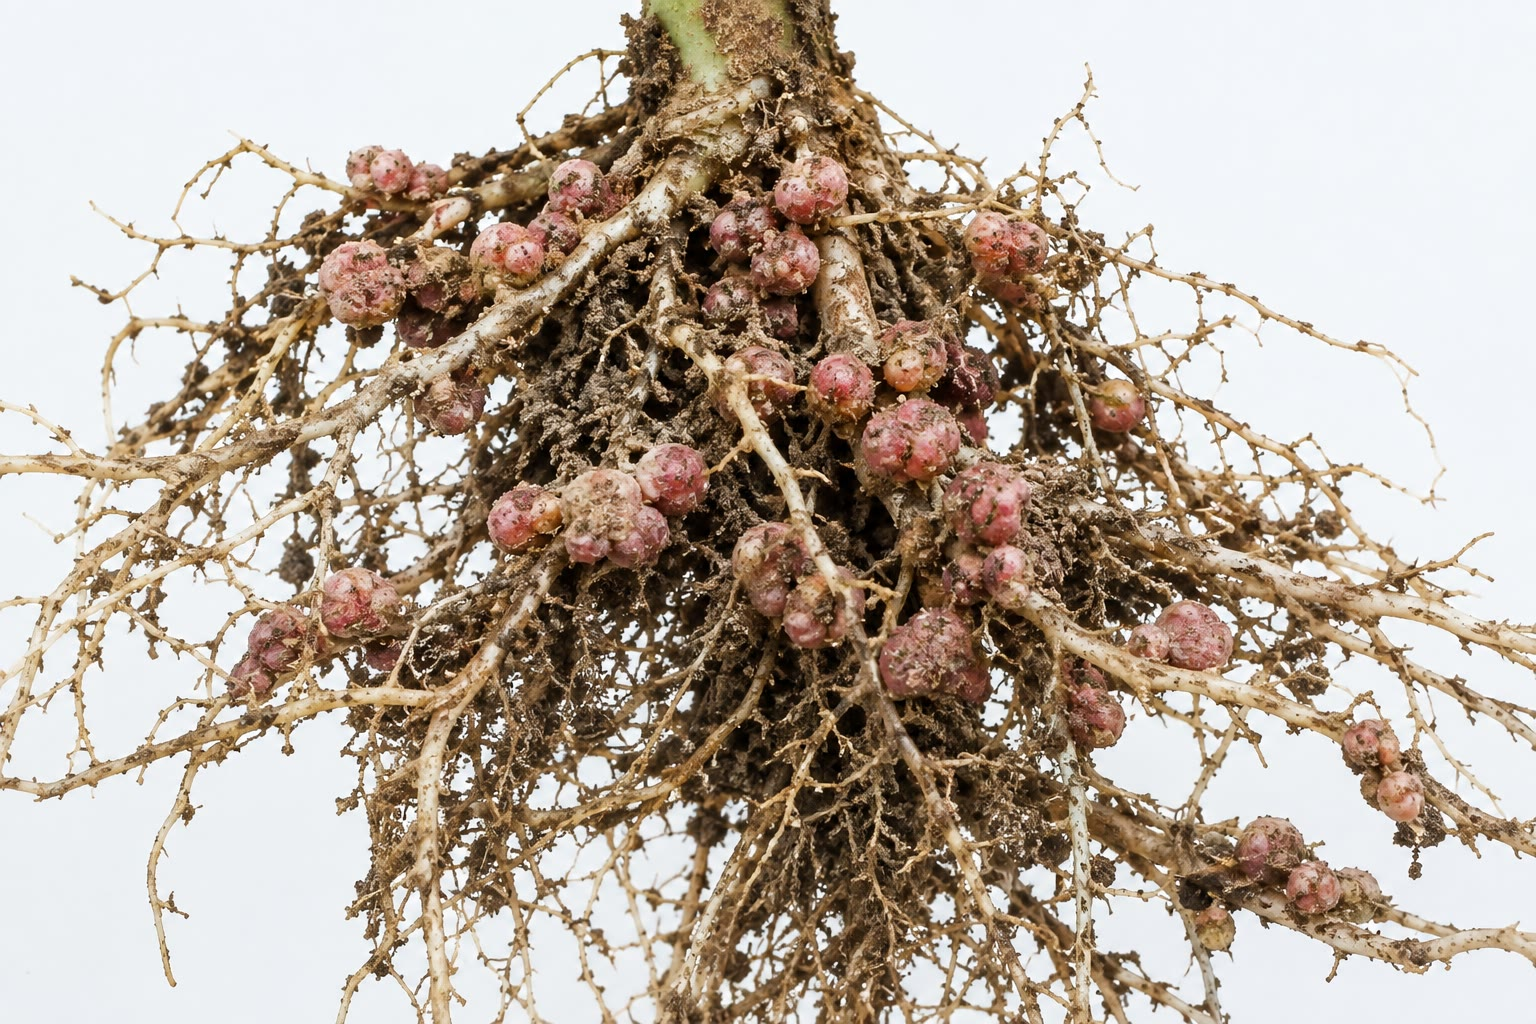
\includegraphics[width=0.46\linewidth]{images/book5/ai/b5-14-root-nodules.jpg}\hspace{0.04\linewidth}
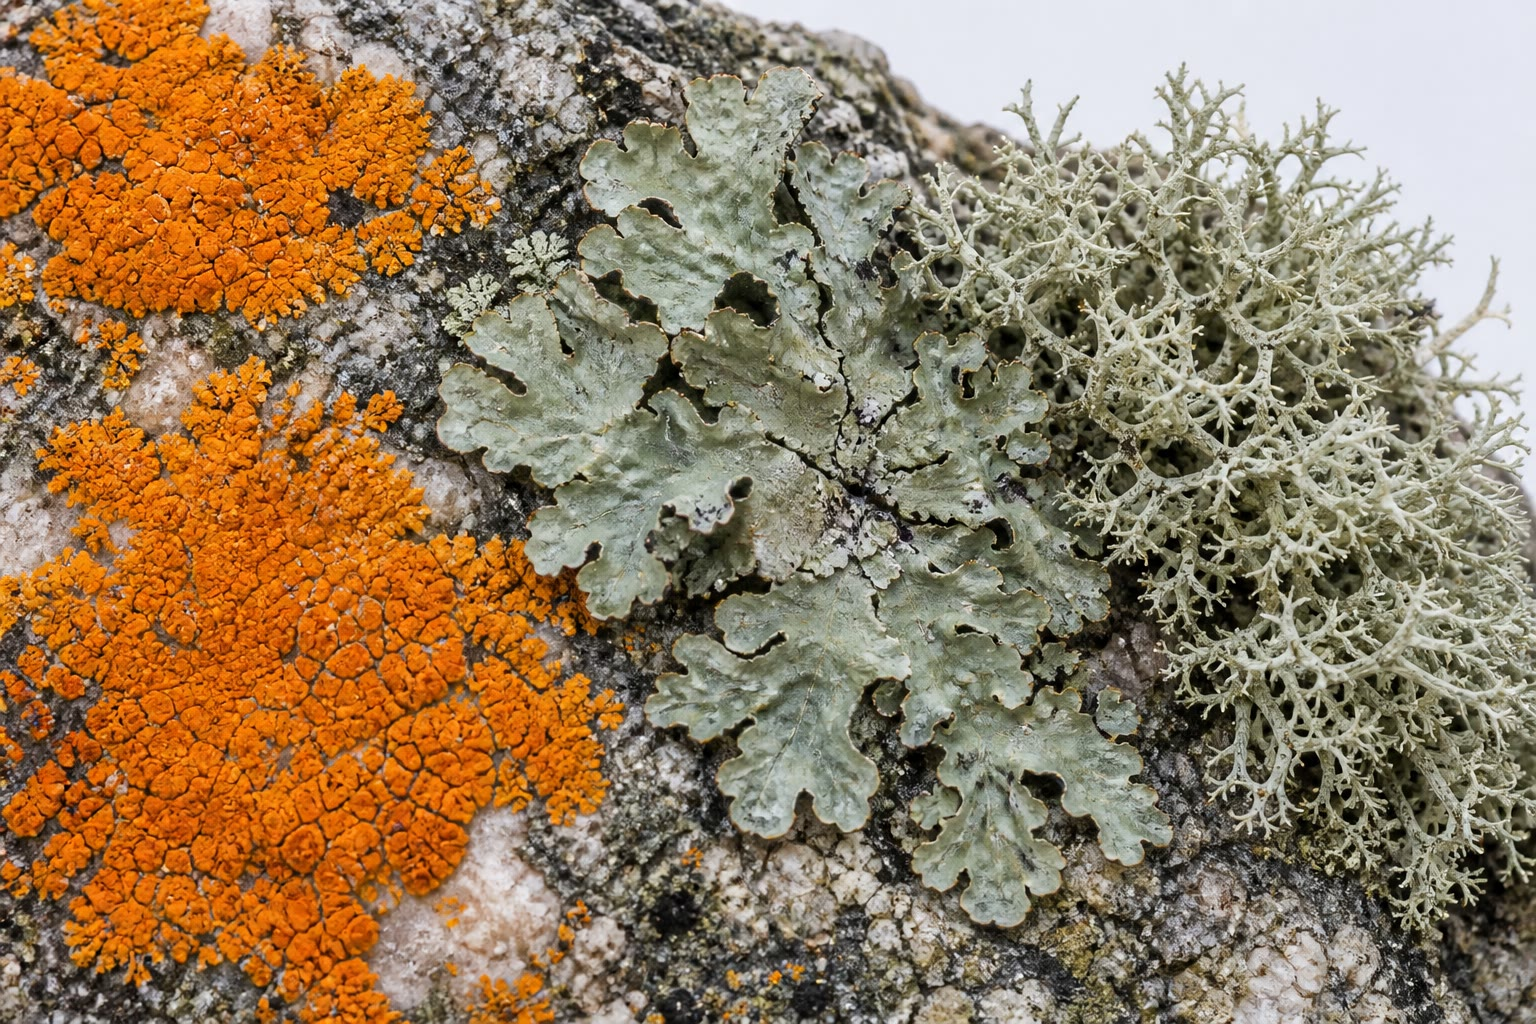
\includegraphics[width=0.46\linewidth]{images/book5/ai/b5-14-lichen.jpg}

{\small Left: the nodulated roots of a legume, each pink nodule a
nitrogen factory of bacteroids fed with sugar. Right: lichens on rock
--- each a fungus housing a photosynthetic alga or cyanobacterium,
together colonising a surface neither could hold alone.}
\end{omfigure}

\section{Partnerships in the sea and elsewhere}

\begin{definition}[Coral and alga]\label{def:b3:microbiomes:coral}
\index{coral symbiosis}\index{zooxanthellae}\index{coral bleaching}
Reef-building corals house dinoflagellate algae (\emph{Symbiodiniaceae},
the \emph{zooxanthellae}) inside the cells of their gut lining, a
million or more per square centimetre. The algae photosynthesise in
the animal's tissue, using the animal's waste CO$_{2}$, ammonia and
phosphate, and pass back up to \qty{90}{\%} of their fixed carbon as
glycerol, sugars and amino acids, which feed the coral and the
calcification that builds the reef; the coral, in turn, controls the
algae's nitrogen supply and hence their growth. The partnership works
within a narrow thermal window: when the water stays about one to two
degrees above the summer maximum for a few weeks, the algae's
photosynthesis is damaged, they release reactive oxygen into the host
cells, and the coral expels them --- \emph{bleaching}, the white
skeleton showing through the translucent animal. A bleached coral
starves; it recovers if the water cools within weeks and dies if not.
The frequency of bleaching has risen fivefold since 1980, and it is the
mechanism by which warming is removing reefs.
\end{definition}

\begin{example}[Symbioses that make habitats]\label{ex:b3:microbiomes:habitats}
A \emph{lichen} is a fungus housing a green alga or a cyanobacterium,
the fungus providing structure, water retention and minerals dissolved
from rock, the photobiont providing sugar (and, if a cyanobacterium,
nitrogen); lichens cover about \qty{8}{\%} of the land surface,
colonise bare rock, and begin its conversion to soil. The tube worm
\emph{Riftia} of the deep-sea vents has no mouth or gut as an adult;
it houses sulfide-oxidising bacteria in a trophosome and delivers them
sulfide and oxygen on a haemoglobin that binds both, growing at over a
metre a year in the dark on chemical energy. Termites digest wood with
a gut community of protists and bacteria, and ruminants digest grass
with a rumen the size of a bathtub in which bacteria, archaea and
fungi ferment cellulose to fatty acids and methane; the cow lives on
the fatty acids and on the bodies of the microbes themselves. In every
case a metabolic capacity --- photosynthesis, nitrogen fixation,
sulfide oxidation, cellulose digestion --- that the host lineage never
evolved has been acquired by partnership in one step.
\end{example}

\begin{omfigure}
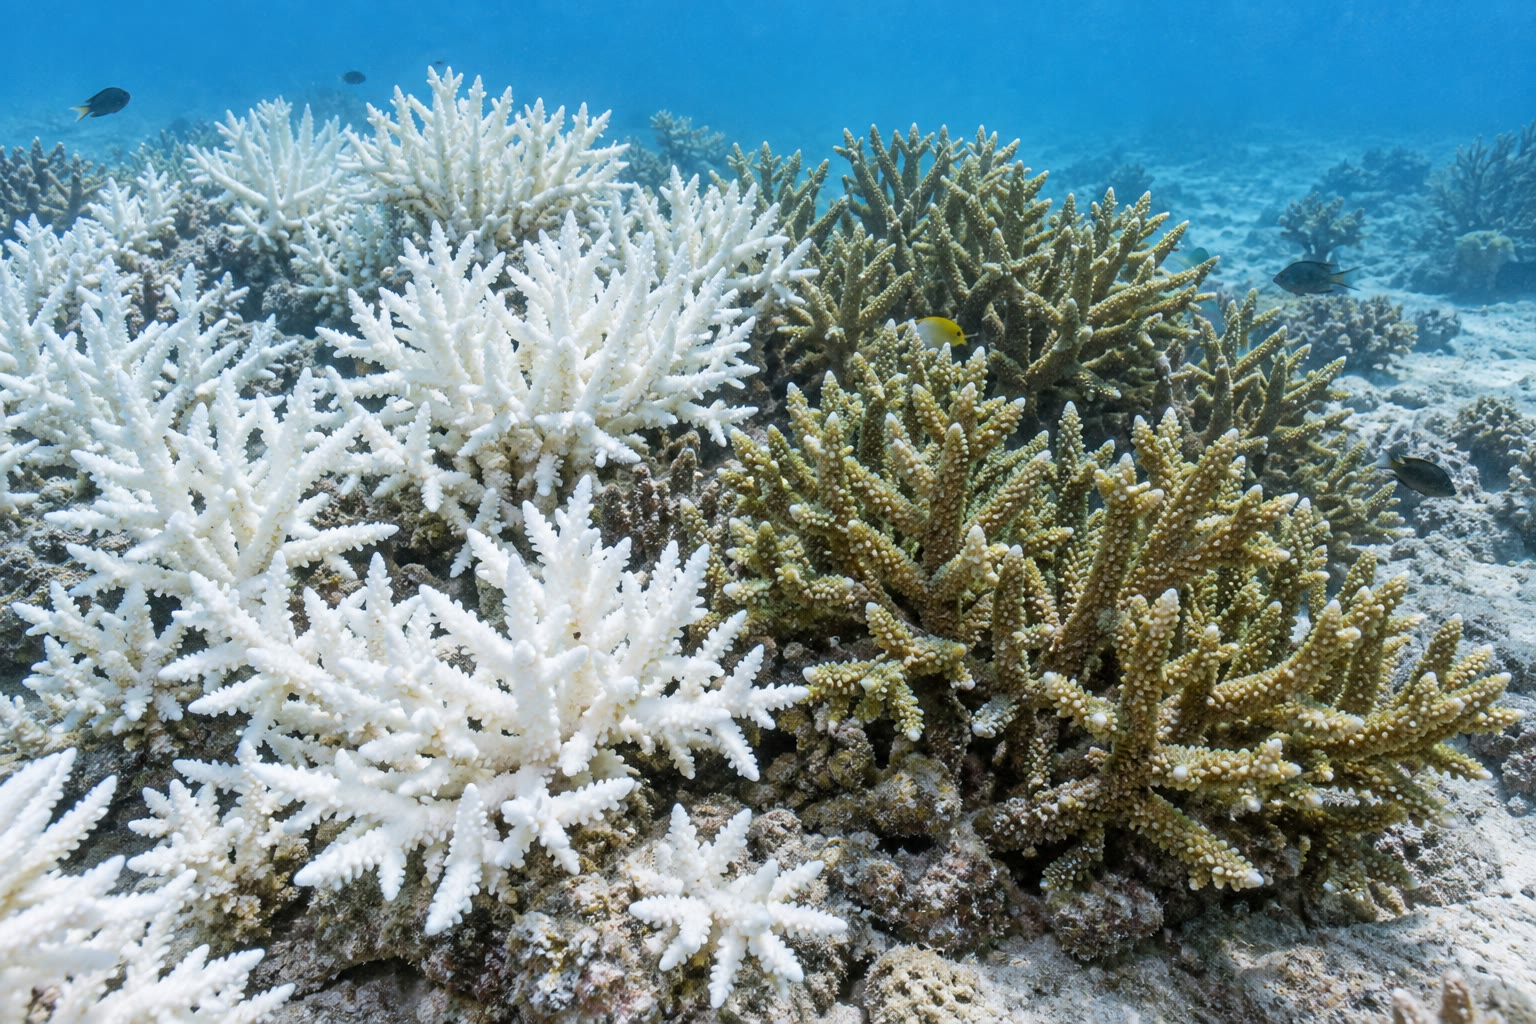
\includegraphics[width=0.56\linewidth]{images/book5/ai/b5-14-coral-bleaching.jpg}

{\small A reef half bleached: the white colonies have expelled their
algae after weeks of water too warm; the brown ones still hold theirs.
The white coral is alive and starving, and has weeks to be recolonised.}
\end{omfigure}

\begin{omfigure}
\begin{tikzpicture}[every node/.style={font=\scriptsize}, >=stealth]
  % coral cell with alga
  \draw[very thick, omDef, fill=omDef!8] (0,0) ellipse (3.2 and 2.0); \node[above] at (0,2.05) {coral cell (gastroderm)};
  \draw[thick, omMeth!70!black, fill=omMeth!30] (-0.4,-0.1) circle (1.05); \node[align=center] at (-0.4,-0.1) {alga\\(zooxanthella)};
  % exchanges
  \draw[->, thick, omMeth!70!black] (0.5,0.4) -- (1.9,0.9) node[right, align=left] {glycerol, sugars, amino acids:\\up to \qty{90}{\%} of fixed carbon};
  \draw[<-, thick, omThm] (0.5,-0.5) -- (1.9,-1.0) node[right, align=left] {CO$_2$, NH$_3$, phosphate\\(the animal's wastes)};
  \draw[<-, thick, omProp] (-1.3,0.3) -- (-2.6,1.0) node[left, align=right] {light through\\the tissue};
  \node[below, align=center] at (1.5,-2.1) {stress: warm water for weeks $\to$ photosynthesis damaged,\\reactive oxygen $\to$ alga expelled $\to$ bleaching};
  % thermometer-like bar on the right
  \begin{scope}[xshift=7.6cm, yshift=-1.6cm]
    \draw[thick] (0,0) rectangle (0.5,3.2);
    \fill[omDef!40] (0,0) rectangle (0.5,2.0); \fill[omProp!60] (0,2.0) rectangle (0.5,2.6); \fill[omThm!60] (0,2.6) rectangle (0.5,3.2);
    \node[right] at (0.6,1.0) {normal range}; \node[right] at (0.6,2.3) {$+\qty{1}{\celsius}$: stress}; \node[right, align=left] at (0.6,2.9) {$+\qty{2}{\celsius}$ for weeks:\\bleaching};
    \node[below, align=center] at (0.25,-0.1) {summer sea\\temperature};
  \end{scope}
\end{tikzpicture}

{\small The coral--alga exchange: the alga fixes carbon with the
animal's wastes and light through its tissue and returns most of it as
food; a small, sustained rise in temperature breaks the partnership.}
\end{omfigure}

\section{From partner to organelle}

\begin{proposition}[Genome reduction and the road to the organelle]\label{prop:b3:microbiomes:reduction}
\index{genome reduction}\index{endosymbiotic gene transfer}
An endosymbiont inherited through the egg lives in a population of a
few cells that never recombine with outsiders. Selection on it is weak
(\cref{ch:b3:molecular-evolution}: a small population fixes slightly
harmful mutations by drift), genes whose products the host supplies are
not missed when they break, and a lost gene is never regained. The
genome therefore shrinks, generation after generation --- \emph{Buchnera}
to \qty{640}{kb}, some insect symbionts to \qty{140}{kb} and a few
hundred genes, the mitochondrion to \qty{16}{kb} and thirteen proteins
in humans --- and the host's nucleus acquires copies of symbiont genes
by \emph{\omterm{prop:b3:microbiomes:reduction}{endosymbiotic gene transfer}}, whose products are imported
back with a targeting sequence. When the host makes most of the
symbiont's proteins, controls its division, and cannot live without it,
the symbiont has become an organelle. Mitochondria and plastids
travelled this road two billion and one billion years ago
(the Year~1 volume); \emph{Paulinella}'s chromatophore is a third
traveller, a hundred million years along.
\end{proposition}

\begin{remark}[The individual revisited]\label{rem:b3:microbiomes:individual}
An animal or plant is a community with a genome at its centre, most of
whose metabolic repertoire, and much of whose development and
immunity, depends on partners it did not inherit in its own DNA. The
practical consequences are already here: the \omterm{def:b3:microbiomes:symbiosis}{microbiome} as a drug
(faecal transplant), as a target of drugs (\omterm{def:b3:bacteriology:antibiotics}{antibiotics}' collateral
damage, dietary fibre as a prescription), as a diagnostic, and as a
route --- through engineered symbionts and \emph{Wolbachia}-carrying
mosquitoes --- to changing the biology of wild populations. The
theoretical one is that natural selection acts on partnerships, and
that the strongest partnerships are those in which one partner's fate
is the other's.
\end{remark}

\section{Exercises}

\begin{exercise}[$\star$]\label{exo:b3:microbiomes:1}
Define \omterm{def:b3:microbiomes:symbiosis}{mutualism}, \omterm{def:b3:microbiomes:symbiosis}{commensalism} and parasitism, and give one example of
each from this chapter. Why can one pair of species move between the
categories?
\end{exercise}

\begin{exercise}[$\star$]\label{exo:b3:microbiomes:2}
Compute $H$, $e^{H}$, $D$ and $1/D$ for a community with abundances
$0.5$, $0.3$, $0.1$, $0.05$, $0.05$.
\end{exercise}

\begin{exercise}[$\star$]\label{exo:b3:microbiomes:3}
Contrast a 16S amplicon survey and shotgun metagenomics: what does each
report, and what can each not tell you?
\end{exercise}

\begin{exercise}[$\star$]\label{exo:b3:microbiomes:4}
List four services the \omterm{def:b3:microbiomes:gut}{gut microbiome} provides to its host and one
disease that follows its disruption.
\end{exercise}

\begin{exercise}[$\star\star$]\label{exo:b3:microbiomes:5}
A sample of $N = 20$ reads holds species with $N_{i} = 10, 6, 3, 1$.
Compute $E[S_{n}]$ for $n = 5$ from the theorem, and \omterm{thm:b3:microbiomes:rarefaction}{Good's coverage}.
\end{exercise}

\begin{exercise}[$\star\star$]\label{exo:b3:microbiomes:6}
The colon holds \qty{400}{g} of contents at $10^{11}$ bacteria per
gram; a bacterium weighs \qty{1}{pg} and its genome has \num{4000}
genes; a person's gut has $1000$ species. Estimate the mass of the
\omterm{def:b3:microbiomes:symbiosis}{microbiome} and the number of distinct genes it carries, and compare
with the human genome's \num{20000}.
\end{exercise}

\begin{exercise}[$\star\star$]\label{exo:b3:microbiomes:7}
Explain the oxygen paradox of the nodule and how \omterm{def:b3:microbiomes:nodule}{leghaemoglobin} and the
diffusion barrier solve it. Why is a nodule pink, and what does a green
nodule mean?
\end{exercise}

\begin{exercise}[$\star\star$]\label{exo:b3:microbiomes:8}
A legume mutant lacks the calcium-spiking component of the \omterm{def:b3:microbiomes:mycorrhiza}{common
symbiosis pathway}. Predict its nodulation and its mycorrhization, and
explain what that says about the evolution of the two symbioses.
\end{exercise}

\begin{exercise}[$\star\star$]\label{exo:b3:microbiomes:9}
Describe Kiers's sanction experiment and what would be predicted if
the plant could not distinguish fixing from non-fixing nodules.
\end{exercise}

\begin{exercise}[$\star\star\star$]\label{exo:b3:microbiomes:10}
Prove that $E[S_{n}]$ in the \omterm{def:b3:microbiomes:diversity}{rarefaction} theorem is an increasing
function of $n$ and reaches $S$ at $n = N$, and show that for a species
with $N_{i} \ll N$ and $n \ll N$ its probability of being seen is about
$1 - (1 - n/N)^{N_{i}}$.
\end{exercise}

\begin{exercise}[$\star\star\star$]\label{exo:b3:microbiomes:11}
\emph{Wolbachia} is transmitted only through eggs. Explain why
selection on it favours female hosts, describe cytoplasmic
incompatibility and show why it lets an infected strain spread even
if infection carries a small cost.
\end{exercise}

\begin{exercise}[$\star\star\star$]\label{exo:b3:microbiomes:12}
Using \cref{prop:b3:microbiomes:reduction}, explain why the genomes of
vertically transmitted endosymbionts shrink but those of free-living
relatives do not, which genes are lost first and which last, and what
would reverse the trend.
\end{exercise}

\section{Problem: The Census of a Gut}

\begin{problem}[{Weekend problem --- a gut microbiome counted in cells,
genes and calories, its diversity measured and rarefied, a legume's
nitrogen budget balanced against its sugar, and a reef's carbon
accounted for, ending on the calories a microbiome earns, the coverage
of a sequencing sample and the sugar a field of beans pays for its
nitrogen}]
\label{pb:b3:microbiomes:1}
Data: colon contents \qty{400}{g} at $10^{11}$ bacteria per gram, cell
mass \qty{1}{pg}; $1000$ species, \num{4000} genes each, \qty{30}{\%}
of genes shared between any two species. Diet: \qty{30}{g} of fibre a
day, fermented to \omterm{def:b3:microbiomes:gut}{short-chain fatty acids} at \qty{10}{mmol} per gram,
each worth \qty{0.9}{kJ}; a diet of \qty{9000}{kJ}. A sequencing sample:
$N = 2000$ reads, $S = 180$ species, $f_{1} = 60$ singletons; abundances
of the top three species $0.30$, $0.20$, $0.10$, the rest evenly spread.
A bean crop fixes \qty{150}{kg} of N per hectare per season and pays
\qty{8}{g} of sugar per gram of N fixed; its photosynthesis yields
\qty{12}{t} of sugar per hectare per season. \omterm{def:b3:microbiomes:nodule}{Nitrogenase}: $16$ ATP per
N$_{2}$. A coral: $10^{6}$ algae per cm$^{2}$, each fixing \qty{20}{pg}
of carbon a day, \qty{90}{\%} passed to the host; the coral tissue
respires \qty{15}{\micro g} of carbon per cm$^{2}$ per day.

\medskip
\noindent\textbf{Part I --- Cells and genes.}
\begin{enumerate}
  \item How many bacteria in the colon, and what do they weigh?
  \item How many bacterial genomes' worth of DNA is that, and how does
        the total compare with the DNA in the $3\times 10^{13}$ human
        cells (\qty{6.4}{pg} each)?
  \item Estimate the number of distinct bacterial genes in the gut,
        allowing for the \qty{30}{\%} overlap (count each species'
        unshared \qty{70}{\%} plus one shared set). Compare with
        \num{20000}.
  \item How many millimoles of \omterm{def:b3:microbiomes:gut}{short-chain fatty acids} does the fibre
        yield per day, how many kilojoules, and what fraction of the
        diet?
  \item A germ-free mouse needs \qty{30}{\%} more food. Is the fatty-acid
        contribution of question 4 enough to explain that? What else
        might?
  \item Bacteria divide in the colon about once a day and the contents
        are voided at the same rate. What steady state does that imply,
        and what happens to the community when a course of \omterm{def:b3:bacteriology:antibiotics}{antibiotics}
        kills \qty{99.9}{\%} of the cells?
\end{enumerate}

\medskip
\noindent\textbf{Part II --- Diversity.}
\begin{enumerate}[resume]
  \item Compute the relative abundance of each of the $177$ minor
        species, then the \omterm{def:b3:microbiomes:diversity}{Shannon index} $H$ and $e^{H}$.
  \item Compute the \omterm{def:b3:microbiomes:diversity}{Simpson index} $D$ and $1/D$. Why is $1/D$ smaller
        than $e^{H}$?
  \item \omterm{thm:b3:microbiomes:rarefaction}{Good's coverage} of the sample; how many reads belong to unseen
        species per thousand?
  \item A second sample of \num{10000} reads from the same gut yields
        $260$ species. Explain, using the \omterm{def:b3:microbiomes:diversity}{rarefaction} theorem, why
        this is not a contradiction, and what to do before comparing
        the two.
  \item In the theorem, what is the probability that a species with
        $N_{i} = 1$ appears in a subsample of $n = 1000$ from $N =
        2000$? With $N_{i} = 5$?
  \item After \omterm{def:b3:bacteriology:antibiotics}{antibiotics} the same gut shows $60$ species, $H = 2.0$,
        and one species at abundance $0.5$. Compute $e^{H}$ and $D$ and
        describe the community in words.
\end{enumerate}

\medskip
\noindent\textbf{Part III --- The nodule's account.}
\begin{enumerate}[resume]
  \item How much sugar does the crop pay per hectare for its
        \qty{150}{kg} of N, and what fraction of its photosynthesis is
        that?
  \item How many moles of N$_{2}$ is \qty{150}{kg} of N, and how many
        moles of ATP does \omterm{def:b3:microbiomes:nodule}{nitrogenase} spend on it?
  \item At $30$ ATP per glucose respired, how many kilograms of glucose
        does that ATP represent? Compare with the sugar paid; what is
        the rest for?
  \item Industrial ammonia costs about \qty{35}{MJ} per kg of N. Using
        \qty{16}{kJ} per gram of sugar, compare the energy cost of the
        crop's nitrogen with the factory's.
  \item A non-fixing rhizobium enters a nodule. If the plant sanctions
        it by halving its oxygen, and its reproduction falls by half,
        what fraction of the next season's \omterm{def:b3:microbiomes:nodule}{rhizobia} are cheaters if
        they began at \qty{10}{\%} and fixers reproduce normally?
        (One round.)
  \item Without sanctions, cheaters that save the cost of fixing
        reproduce \qty{20}{\%} more. Over ten seasons, what fraction are
        cheaters, from the same start? What does the comparison show?
\end{enumerate}

\medskip
\noindent\textbf{Part IV --- The reef's account.}
\begin{enumerate}[resume]
  \item How much carbon do the algae of one square centimetre fix per
        day, and how much reaches the coral?
  \item Compare with the coral's respiration. What is the surplus, and
        what is it used for?
  \item After bleaching, \qty{95}{\%} of the algae are gone. Recompute the
        carbon supplied. How long can the coral last on reserves of
        \qty{300}{\micro g} of carbon per cm$^{2}$?
  \item The stress is often measured in degree-heating-weeks: the sum,
        over the season, of the weekly excess above the summer
        maximum. Eight weeks at $+\qty{1}{\celsius}$ or four at
        $+\qty{2}{\celsius}$ both give $8$; bleaching begins near $4$.
        Which of the two profiles is worse, and why might the metric
        nevertheless work?
  \item Corals can host several algal species with different thermal
        limits. Propose how a reef might adapt, and what limits that.
  \item A reef of \qty{1}{km^2} of living coral surface: how much
        carbon do its algae fix per day and per year, in tonnes?
  \item Summarise: the fraction of the diet supplied by the \omterm{def:b3:microbiomes:symbiosis}{microbiome}
        (question~4), the coverage of the sequencing sample
        (question~9), and the fraction of photosynthesis a bean crop
        pays for its nitrogen (question~13).
\end{enumerate}
\end{problem}
